Para la toma de datos se consideraron dos escenarios: el primero el Laboratorio de Robótica 0L3 del Instituto de Computación Científica Avanzada de la Universidad de Extremadura (ICCAEx), situado en los Institutos Universitarios de Investigación de la Universidad de Extremadura en Badajoz, en el que se disponía de una superficie amplia y libre de objetos para tomar medidas en un escenario lo más cercano a lo ideal.

El segundo escenario fue la segunda planta del edificio B de la Facultad de Física de la Universidad de Extremadura, elegido para acercarse a una disposición más general, con obstáculos entre las balizas y el objetivo.

\subsection{Simulación previa}

Antes de proceder a la toma de medidas en las dos localizaciones escogidas se escribió el código responsable de los nodos de ROS que desplazaban al robot y recogían los datos de posicionamiento con la ayuda del simulador Stage.
Todo este código y su estructura figura en el Apéndice 2.

Además de el código del nodo, también es necesario construir el mapa sobre el que la navegación del robot construye el planner global y así conocer la posición y el movimiento del robot.
En el caso del laboratorio, dicho mapa estaba ya construido al ser localización habitual de investigación con el Turtlebot.

No fue así en para el edificio de Física.
En una primera instancia se recurrió a los planos de construcción, a la espera de posibles correcciones con la obtención de las dimensiones reales de la planta con un medidor láser.

Finalmente estas correcciones fueron necesarias, ya que los planos no respetaban completamente las medidas reales de los pasillos de la planta que debía recorrer el robot.

\begin{figure}[H]
  \centering
  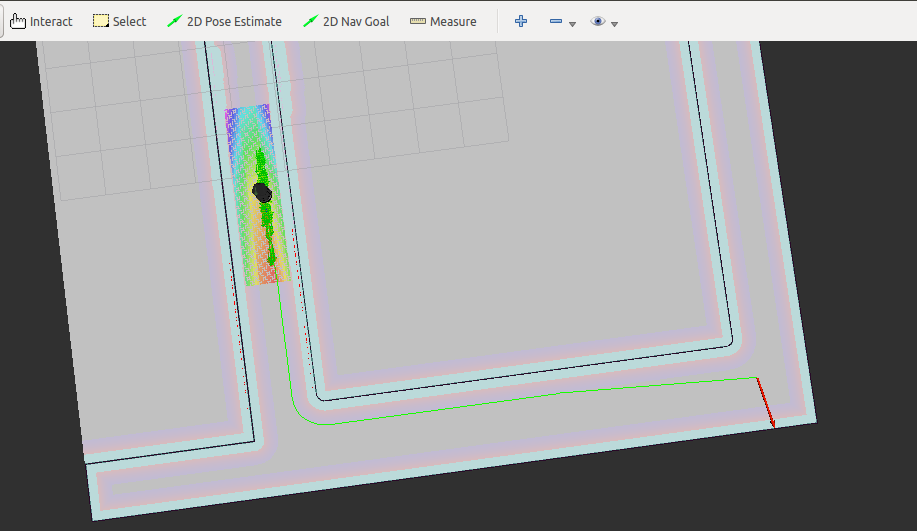
\includegraphics[width=0.75\textwidth]{pic/Trayectoria.png}
  \caption{Captura de \textit{rviz} con el primer mapa del edificio de Física, sin columnas.}
  \label{fig:plano_fisica}
\end{figure}

Además, por simplicidad la primera aproximación del mapa no incluía las columnas de la planta, como se puede observar en la Figura \ref{fig:plano_fisica}.
Aunque la superficie que ocupan en el plano es pequeña, una primera toma de medidas con el robot hizo evidente que su reconocimiento por parte de los sensores que incorpora llevaba a las rutinas de posicionamiento local a equívocos a la hora de relacionar estas columnas con las paredes del mapa proporcionado.
Esto hacía que los valores obtenidos por el posicionamiento local del robot tuviesen discrepancias de hasta 50cm respecto a la posición real, medida de forma manual.

Por ello se procedió a crear un nuevo mapa con dichas columnas.
En este caso el posicionamiento del robot mejoró de forma significativa, siendo capaz de identificar las columnas con solvencia y reduciendo las discrepancias observadas a unos 10cm, mismos valores que se obtenían en el laboratorio.

\subsection{Toma de medidas}

En todos los casos la toma de medidas siguió el mismo procedimiento: en base a una trayectoria fijada que atraviesa una serie de puntos en cada escenario se toman un número prefijado de datos a partir de los sensores, con el robot parado en cada uno de dichos puntos.

Para determinar el número de valores a recoger en cada caso se realizaron tomas de medidas previas para determinar la naturaleza de los datos obtenidos.
En todos los casos se obtuvo una distribución de tipo gaussiano, como se puede ver en la figura \ref{fig:datos_sensor}, por lo que se tomaron 50 datos en el caso del laboratorio y 250 en el caso del edificio de Física con el objetivo tener una dispersión al menos menor de 2cm tomando el mínimo número de datos.

\begin{figure}[H]
  \begin{subfigure}[b]{.5\textwidth}
    \centering
    \begin{tikzpicture}
\begin{axis}[width = \textwidth, height = 0.9\textwidth,ymin=0,xlabel={Posicion (cm)}]
    \addplot [hist={bins=10,data=x}, fill=black!50]
    table {data/ejemplo_sensores.txt};
    % table [x index=0, y index=1, z index=3] {data/ejemplo_sensores.txt};
\end{axis}
\end{tikzpicture} 
    \caption{Eje $x$}
    \label{fig:hist_x}
  \end{subfigure}
  \begin{subfigure}[b]{.5\textwidth}
    \centering
    \begin{tikzpicture}
\begin{axis}[width = \textwidth, height = 0.9\textwidth,ymin=0,xlabel={Posicion (cm)}]
    \addplot [hist={bins=10,data=y}, fill=black!50]
    table {data/ejemplo_sensores.txt};
    % table [x index=0, y index=1, z index=3] {data/ejemplo_sensores.txt};
\end{axis}
\end{tikzpicture}
    \caption{Eje $y$}
    \label{fig:hist_y}
  \end{subfigure}
  \caption{Histograma de los datos de posicionamiento de los sensores en uno de los puntos del edificio de Física, con un ajuste a una curva gaussiana en cada caso.}
  \label{fig:datos_sensor}
\end{figure}

Además, para eliminar cualquier tipo de anomalía estadística cada trayectoria se repitió un mínimo de tres veces, tras las que se evaluaron los datos.
En los casos en los que la dispersión fue excesiva, se procedió a repetir de nuevo estas mediciones.

En las primeras tomas, donde se orientaba el robot hacia el siguiente punto de tal forma que su desplazamiento tomase el menor tiempo posible, se observó que el diseño de las antenas de los sensores utilizados, con una ganancia ligeramente dependiente del ángulo de incidencia \cite{ang}, hacía que, al girar el sensor asignado como objetivo, la estimación de su posición variase.

Esta observación también ha sido recogida en trabajos previos \cite{MSTesis}, donde se intentaba corregir a partir de medidas con distintos ángulos de incidencia.
Esto no es posible en el caso de este trabajo, ya que no versa sobre el desarrollo de un algoritmo de posicionamiento, sino sobre el estudio la precisión del ya implementado.
El algoritmo utilizado es propiedad de la empresa fabricante de los sensores, que no ha liberado detalles sobre su implementación, lo que hace imposible cualquier corrección.

Así, para minimizar este obstáculo todas las medidas que figuran en los resultados están tomadas colocando al robot con el mismo ángulo respecto a las balizas, de tal manera que no es necesario considerar variaciones en la posición obtenida debido a su orientación.

\subsection{Laboratorio de Robótica del ICCAEx}

La primera toma de medidas tuvo lugar en el laboratorio 0L3 del ICCAEx, donde se disponía de una superficie de aproximadamente 5 metros por 7 metros completamente libre para usar por el robot como se puede ver en la Figura \ref{fig:foto_lab}.

\begin{figure}[H]
  \begin{subfigure}[b]{.5\textwidth}
    \centering
    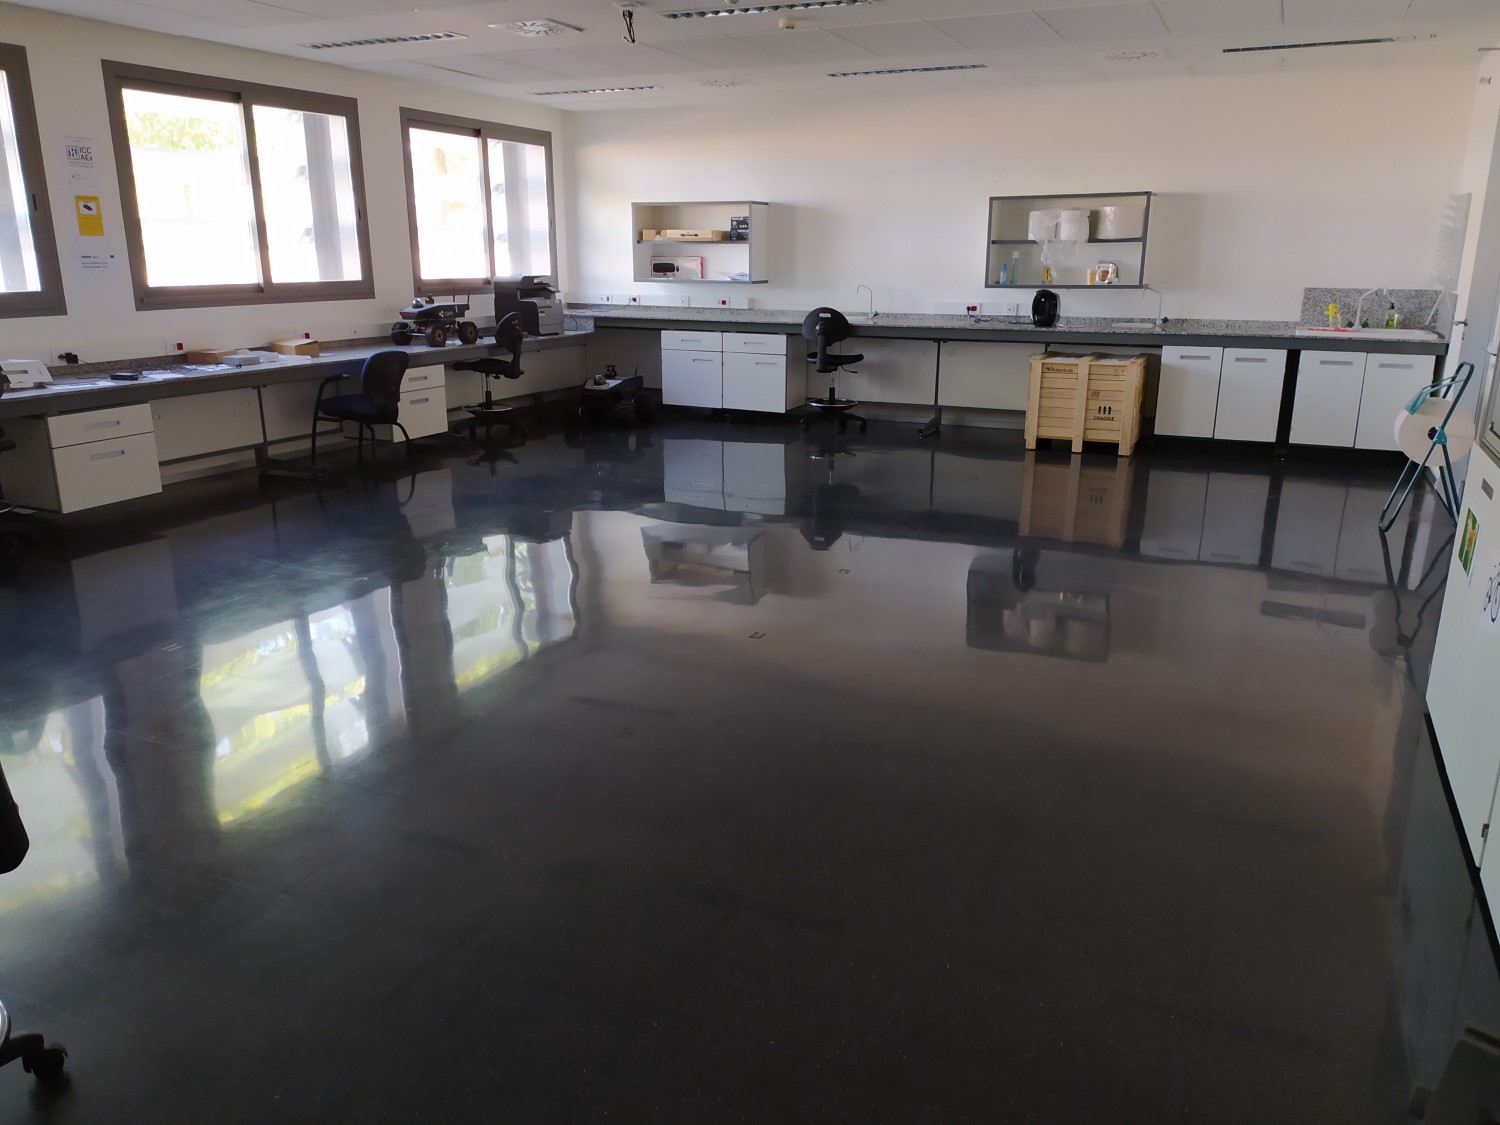
\includegraphics[width=0.9\textwidth]{pic/lab1.jpg}
    % \caption{Eje x}
    \label{fig:foto_lab1}
  \end{subfigure}
  \begin{subfigure}[b]{.5\textwidth}
    \centering
    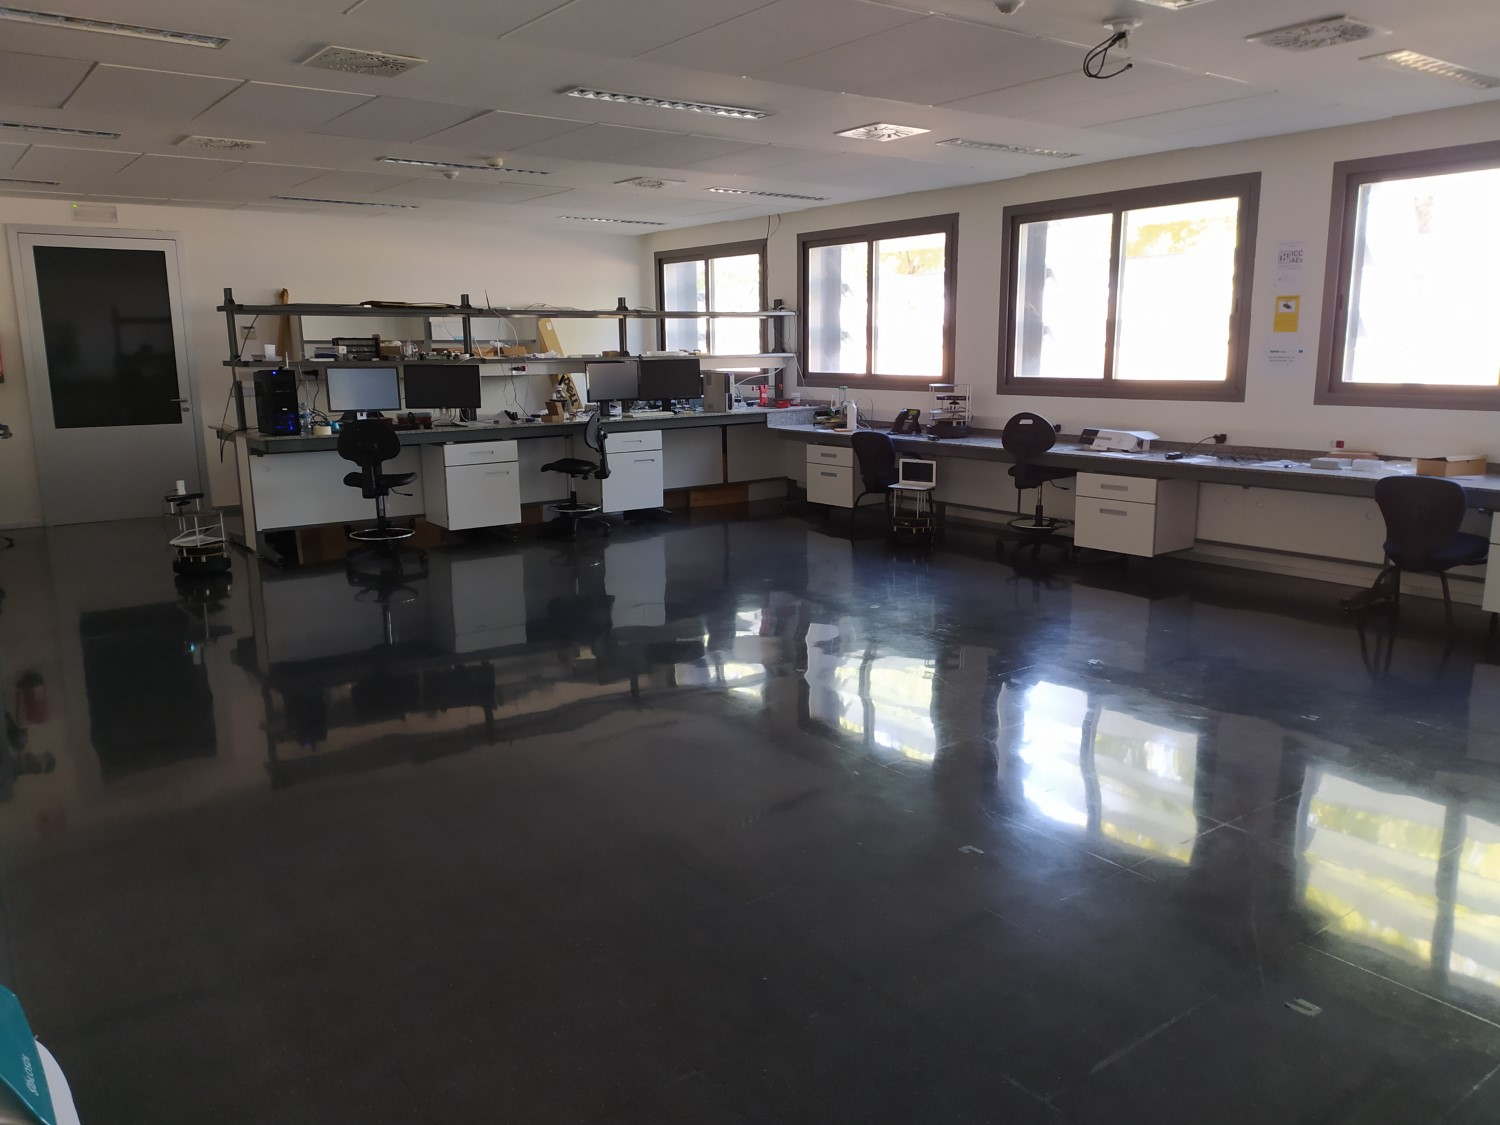
\includegraphics[width=0.9\textwidth]{pic/lab2.jpg}
    % \caption{Eje y}
    \label{fig:foto_lab2}
  \end{subfigure}
  \caption{Fotografías del laboratorio de Robótica del ICCAEx.}
  \label{fig:foto_lab}
\end{figure}

Debido a la libertad a la hora de recorrer dicha superficie se eligieron tres trayectorias que cubriesen todos los puntos a evaluar, establecidos en una cuadrícula con una separación de 1 metro entre cada uno de ellos de tal forma que se evitase un posible sesgo en el movimiento del robot.

\begin{figure}[H]
    \begin{subfigure}[b]{.3\textwidth}
      \centering
      \def\svgwidth{0.8\linewidth}
	    \input{./fig/lab.pdf_tex} 
      \caption{Puntos a evaluar}
      \label{fig:puntos}
    \end{subfigure}
    \begin{subfigure}[b]{.3\textwidth}
      \centering
      \def\svgwidth{0.8\linewidth}
	    \input{./fig/lab_espiral.pdf_tex} 
      \caption{Trayectoria en espiral}
      \label{fig:espiral}
    \end{subfigure}
    \begin{subfigure}[b]{.3\textwidth}
        \centering
        \def\svgwidth{0.8\linewidth}
	    \input{./fig/lab_vertical.pdf_tex} 
        \caption{Trayectoria en vertical}
        \label{fig:vertical}
      \end{subfigure}
    \caption{Disposición del laboratorio.}
    \label{fig:laboratorio}
\end{figure}

La primera de estas trayectorias tenía un recorrido con origen en el centro del laboratorio, acercándose a las paredes exteriores en forma de espiral, con algunas modificaciones para asegurar el paso por todos los puntos.

El segundo trayecto hacía que el robot avanzase de forma recta siguiendo líneas verticales --en el sentido tal y como se ha planteado la representación en dos dimensiones en la figura \ref{fig:vertical}--, con separación de un metro entre cada punto.

Por último se diseñó una trayectoria en la que robot pasase de forma aleatoria por los 35 puntos a medir, de tal forma que en cada intento el orden fuese distinto.

Para comprobar en este escenario ideal el efecto de la colocación de las balizas se repitió la toma de medida en dos configuraciones, colocando 4 y 6 sensores respectivamente.
Teniendo en cuenta que el sistema empleado solo utiliza cuatro de las balizas para el posicionamiento del objetivo, el uso de la configuraciones con 6 de los sensores solo afecta a la posición de dichas baliza en los cálculos, usando siempre los cuatro sensores más cercanos.

La altura a la que fueron colocadas los sensores que actúan como balizas se vio restringida por el mobiliario del laboratorio, de modo que la mayoría se encontraban a unos 180cm del suelo con una de ellas a 80cm y otra a 200cm, aunque el sistema de los sensores permite estas diferencias de alturas en el modo de configuración manual de las balizas.

En la figura \ref{fig:lab_sensores} es posible comprobar la posición respecto a los puntos de medida de las balizas en ambas configuraciones.

\begin{figure}[H]
  \begin{subfigure}[b]{.5\textwidth}
    \centering
    \def\svgwidth{0.7\linewidth}
    \input{./fig/lab_4sensores.pdf_tex} 
    \caption{4 balizas}
    \label{fig:lab_4sens}
  \end{subfigure}
  \ \
  \begin{subfigure}[b]{.5\textwidth}
    \centering
    \def\svgwidth{0.82\linewidth}
    \input{./fig/lab_6sensores.pdf_tex}  
    \caption{6 balizas}
    \label{fig:lab_6sens}
  \end{subfigure}
  \caption{Configuraciones de las balizas en el laboratorio.}
  \label{fig:lab_sensores}
\end{figure}

\subsection{Edificio de la Facultad de Física}

El segundo escenario se encontraba en la primera planta del edificio B de la Facultad de Física, en la que por razones estructurales se encuentran una serie de columnas como se puede observar en la Figura \ref{fig:foto_fisica}.

En este escenario aparecen elementos más cercanos a una implementación de un sistema de posicionamiento local habitual: obstáculos en las balizas, que no es posible colocar en cualquier lugar, y un tránsito de personas habitual que podía interferir en la señal del sistema utilizado.

\begin{figure}[H]
  \begin{subfigure}[b]{.5\textwidth}
    \centering
    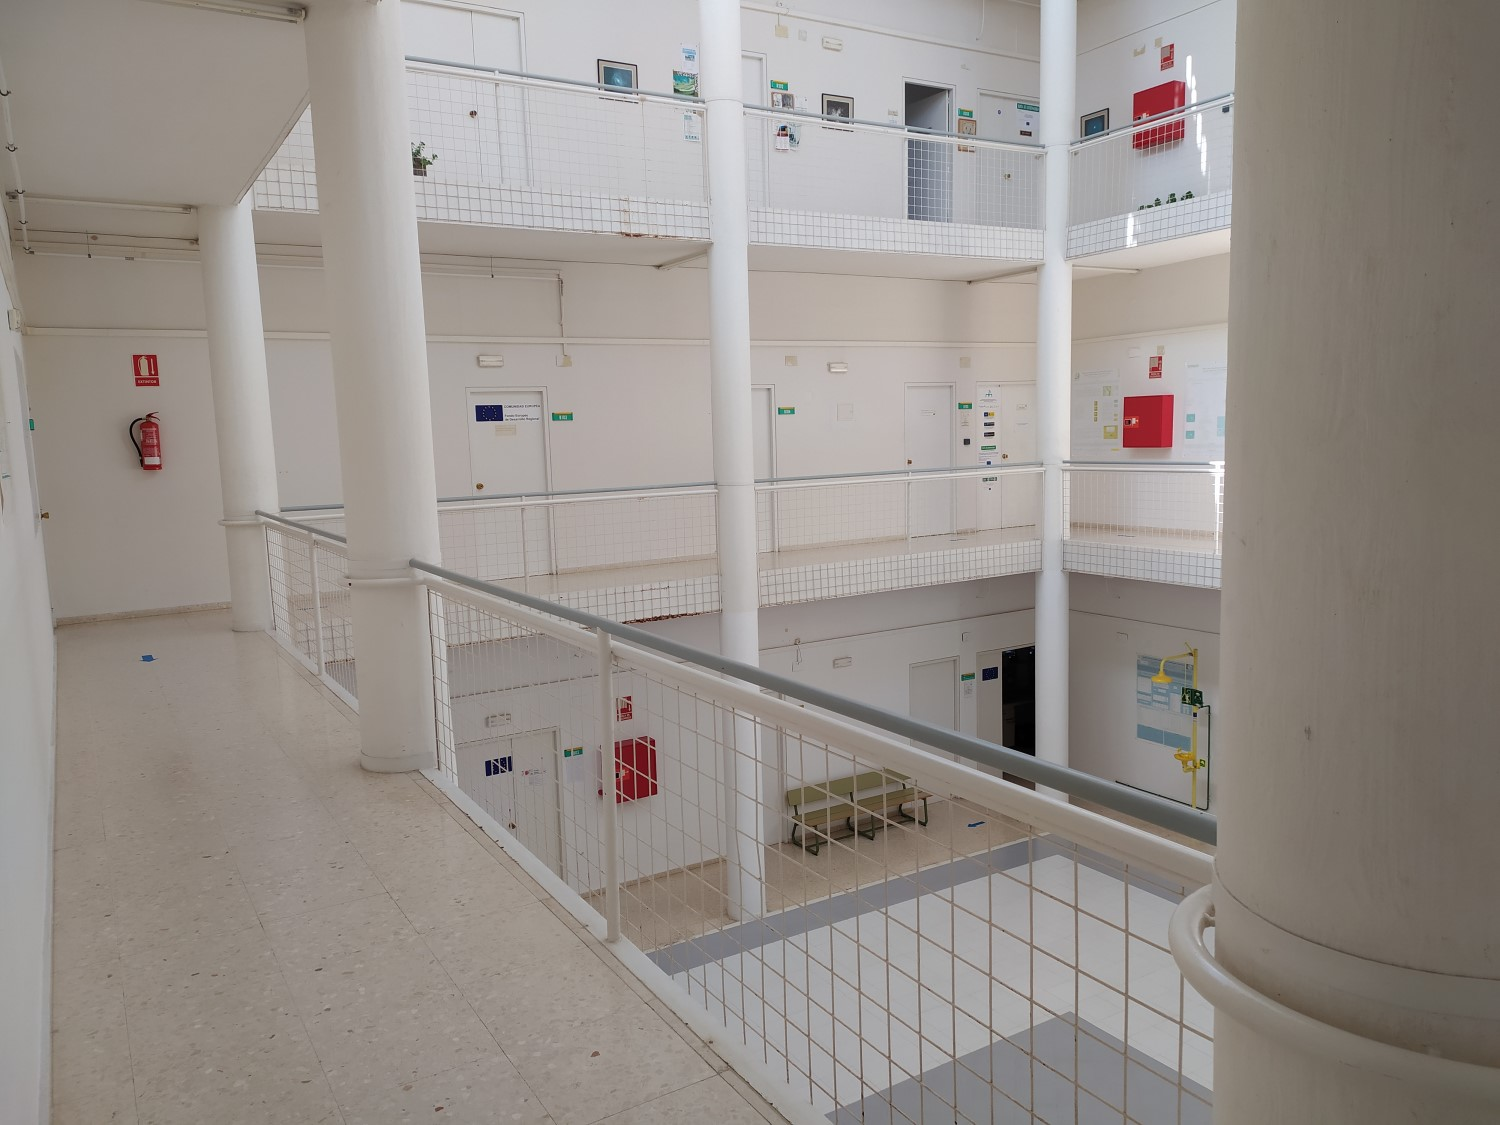
\includegraphics[width=0.9\textwidth]{pic/fisica1.jpg}
    % \caption{Eje x}
    \label{fig:foto_fisica1}
  \end{subfigure}
  \begin{subfigure}[b]{.5\textwidth}
    \centering
    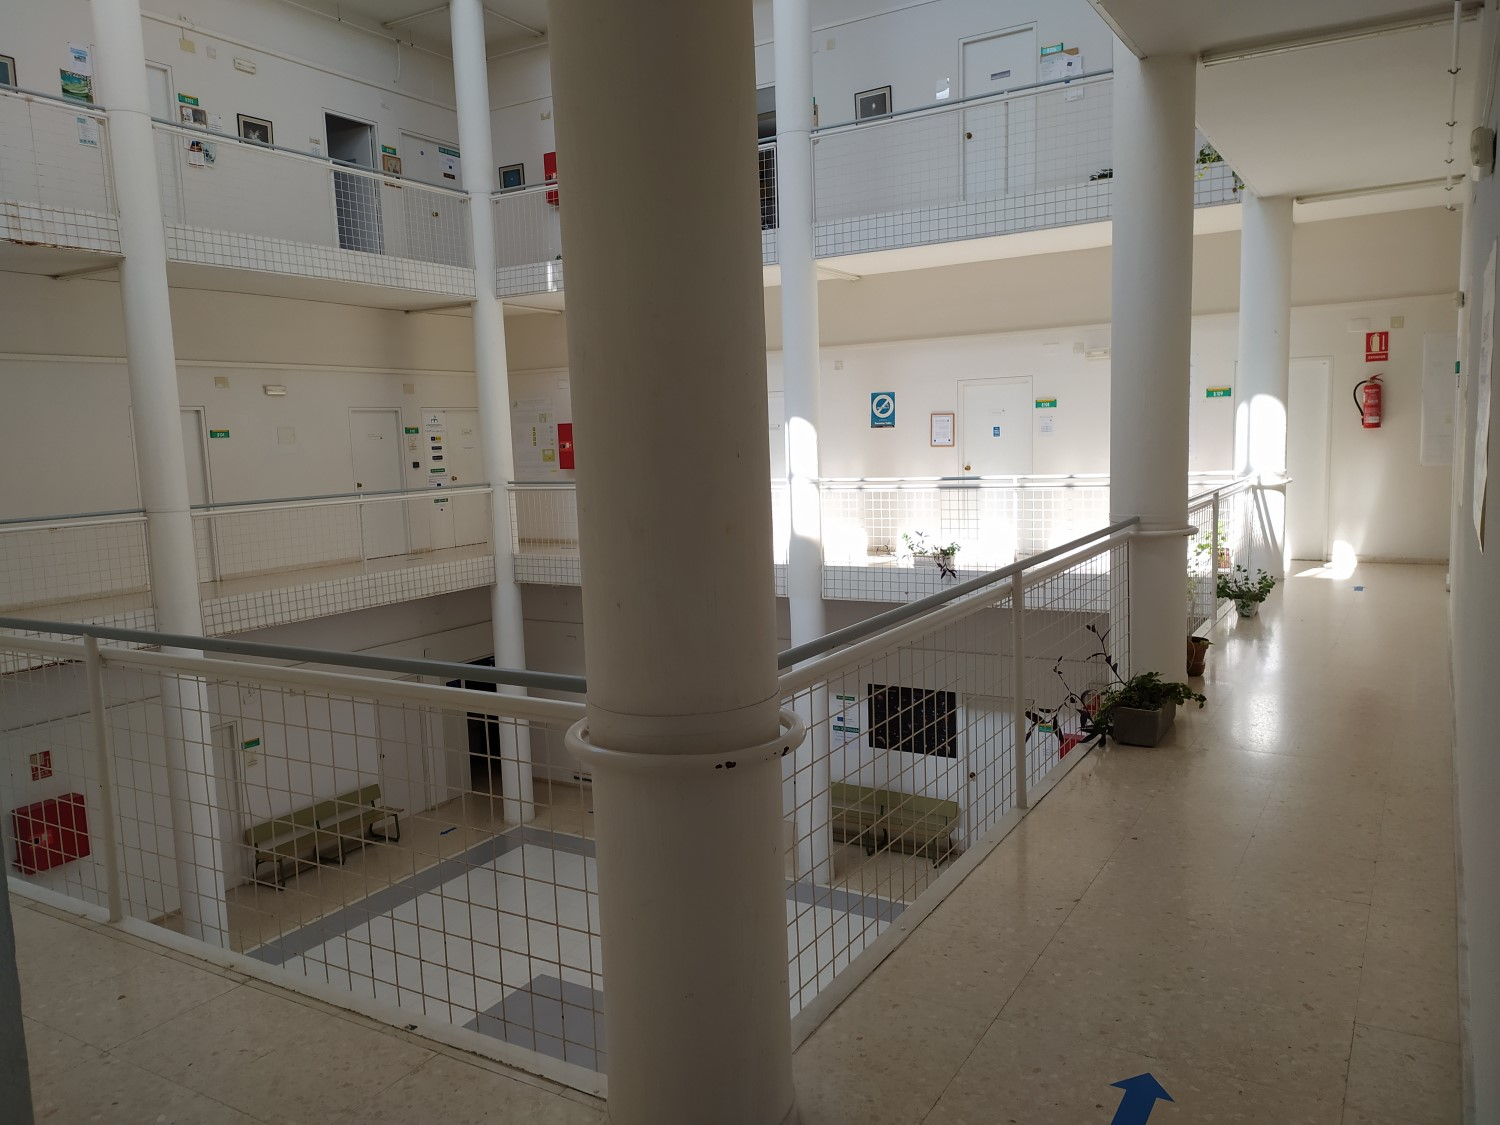
\includegraphics[width=0.9\textwidth]{pic/fisica2.jpg}
    % \caption{Eje y}
    \label{fig:foto_fisica2}
  \end{subfigure}
  \caption{Fotografías del edificio B de la Facultad de Física.}
  \label{fig:foto_fisica}
\end{figure}

En este caso todas las medidas fueron tomadas utilizando la misma trayectoria, que se puede observar en la Figura~\ref{fig:fisica}, que seguía los pasillos de la planta del edificio al no poder optar a más variaciones.

\begin{figure}[H]
  \begin{subfigure}[b]{.5\textwidth}
    \centering
    \def\svgwidth{0.75\linewidth}
    \input{./fig/fisica_num.pdf_tex} 
    \caption{Puntos a evaluar}
    \label{fig:puntos_fisica}
  \end{subfigure}
  \begin{subfigure}[b]{.5\textwidth}
    \centering
    \def\svgwidth{0.75\linewidth}
    \input{./fig/fisica_tray.pdf_tex} 
    \caption{Trayectoria}
    \label{fig:trayecto_fisica}
  \end{subfigure}
  \caption{Disposición de la planta del edificio de Física.}
  \label{fig:fisica}
\end{figure}

Al igual que en el caso del laboratorio, se repitieron las medidas con distintas configuraciones de las balizas, con tres alternativas en este caso: 4, 6 y 8 balizas repartidas de la forma más uniforme posible tal y como se indica en la figura \ref{fig:sensores_fisica}.

\begin{figure}[H]
  \begin{subfigure}[b]{.3\textwidth}
    \centering
    \def\svgwidth{0.9\linewidth}
    \input{./fig/fisica_4sens.pdf_tex} 
    \caption{4 balizas}
    \label{fig:sensores_fisica_4}
  \end{subfigure}
  \begin{subfigure}[b]{.3\textwidth}
    \centering
    \def\svgwidth{0.9\linewidth}
    \input{./fig/fisica_6sens.pdf_tex}  
    \caption{6 balizas}
    \label{fig:sensores_fisica_6}
  \end{subfigure}
  \begin{subfigure}[b]{.3\textwidth}
    \centering
    \def\svgwidth{0.9\linewidth}
    \input{./fig/fisica_8sens.pdf_tex}  
    \caption{8 balizas}
    \label{fig:sensores_fisica_8}
  \end{subfigure}
  \caption{Configuraciones de las balizas en el edificio de Física.}
  \label{fig:sensores_fisica}
\end{figure}

Como en el caso del laboratorio, el kit de sensores UWB utilizado solo usa 4 de las balizas disponibles para estimar la posición del objetivo, por lo que el número mayor de sensores colocados permite una mayor libertad al elegir las balizas con mejor recepción de la señal pero no afinar la estimación con un número mayor de muestras para determinar la intersección de las curvas que definen.

Como es posible ver en la figura \ref{fig:sensores_fisica} la posición de los sensores no es completamente uniforme, debido a que no toda la superficie de la planta estaba disponible por la disposición de los despachos y laboratorios.
En este caso la altura de todas las balizas fue similar, a 170cm respecto al suelo.